\documentclass[border=4pt]{standalone}

\usepackage{amsmath}
\usepackage{tikz}
\usepackage{mathdots}
\usepackage{yhmath}
\usepackage{cancel}
\usepackage{color}
\usepackage{siunitx}
\usepackage{array}
\usepackage{multirow}
\usepackage{amssymb}
\usepackage{gensymb}
\usepackage{tabularx}
\usepackage{booktabs}
\usetikzlibrary{fadings}
\usetikzlibrary{patterns}


\begin{document}
 
     

\tikzset{every picture/.style={line width=0.75pt}} %set default line width to 0.75pt        

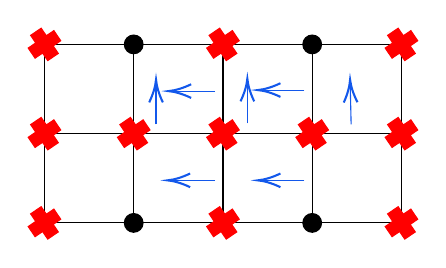
\begin{tikzpicture}[x=0.75pt,y=0.75pt,yscale=-1,xscale=1]
%uncomment if require: \path (0,300); %set diagram left start at 0, and has height of 300

%Shape: Grid [id:dp9478383240032673] 
\draw  [draw opacity=0] (122,139) -- (298.18,139) -- (298.18,230) -- (122,230) -- cycle ; \draw   (122,139) -- (122,230)(165,139) -- (165,230)(208,139) -- (208,230)(251,139) -- (251,230)(294,139) -- (294,230) ; \draw   (122,139) -- (298.18,139)(122,182) -- (298.18,182)(122,225) -- (298.18,225) ; \draw    ;
%Shape: Circle [id:dp1392241818192772] 
\draw  [color={rgb, 255:red, 0; green, 0; blue, 0 }  ,draw opacity=1 ][fill={rgb, 255:red, 0; green, 0; blue, 0 }  ,fill opacity=1 ] (160.5,139) .. controls (160.5,136.51) and (162.51,134.5) .. (165,134.5) .. controls (167.49,134.5) and (169.5,136.51) .. (169.5,139) .. controls (169.5,141.49) and (167.49,143.5) .. (165,143.5) .. controls (162.51,143.5) and (160.5,141.49) .. (160.5,139) -- cycle ;
%Shape: Circle [id:dp2311140486165839] 
\draw  [color={rgb, 255:red, 0; green, 0; blue, 0 }  ,draw opacity=1 ][fill={rgb, 255:red, 0; green, 0; blue, 0 }  ,fill opacity=1 ] (160.5,225) .. controls (160.5,222.51) and (162.51,220.5) .. (165,220.5) .. controls (167.49,220.5) and (169.5,222.51) .. (169.5,225) .. controls (169.5,227.49) and (167.49,229.5) .. (165,229.5) .. controls (162.51,229.5) and (160.5,227.49) .. (160.5,225) -- cycle ;
%Shape: Circle [id:dp3473688645574804] 
\draw  [color={rgb, 255:red, 0; green, 0; blue, 0 }  ,draw opacity=1 ][fill={rgb, 255:red, 0; green, 0; blue, 0 }  ,fill opacity=1 ] (246.5,225) .. controls (246.5,222.51) and (248.51,220.5) .. (251,220.5) .. controls (253.49,220.5) and (255.5,222.51) .. (255.5,225) .. controls (255.5,227.49) and (253.49,229.5) .. (251,229.5) .. controls (248.51,229.5) and (246.5,227.49) .. (246.5,225) -- cycle ;
%Shape: Circle [id:dp869372099178775] 
\draw  [color={rgb, 255:red, 0; green, 0; blue, 0 }  ,draw opacity=1 ][fill={rgb, 255:red, 0; green, 0; blue, 0 }  ,fill opacity=1 ] (246.5,139) .. controls (246.5,136.51) and (248.51,134.5) .. (251,134.5) .. controls (253.49,134.5) and (255.5,136.51) .. (255.5,139) .. controls (255.5,141.49) and (253.49,143.5) .. (251,143.5) .. controls (248.51,143.5) and (246.5,141.49) .. (246.5,139) -- cycle ;
%Shape: Cross [id:dp4851833566528194] 
\draw  [color={rgb, 255:red, 255; green, 0; blue, 0 }  ,draw opacity=1 ][fill={rgb, 255:red, 255; green, 0; blue, 0 }  ,fill opacity=1 ] (126.53,132.38) -- (129.82,137.24) -- (126.18,139.71) -- (128.65,143.35) -- (123.58,146.79) -- (121.11,143.15) -- (117.47,145.62) -- (114.18,140.76) -- (117.82,138.29) -- (115.35,134.65) -- (120.42,131.21) -- (122.89,134.85) -- cycle ;
%Shape: Cross [id:dp2819332325249988] 
\draw  [color={rgb, 255:red, 255; green, 0; blue, 0 }  ,draw opacity=1 ][fill={rgb, 255:red, 255; green, 0; blue, 0 }  ,fill opacity=1 ] (169.53,175.38) -- (172.82,180.24) -- (169.18,182.71) -- (171.65,186.35) -- (166.58,189.79) -- (164.11,186.15) -- (160.47,188.62) -- (157.18,183.76) -- (160.82,181.29) -- (158.35,177.65) -- (163.42,174.21) -- (165.89,177.85) -- cycle ;
%Shape: Cross [id:dp2585290833394436] 
\draw  [color={rgb, 255:red, 255; green, 0; blue, 0 }  ,draw opacity=1 ][fill={rgb, 255:red, 255; green, 0; blue, 0 }  ,fill opacity=1 ] (212.53,132.38) -- (215.82,137.24) -- (212.18,139.71) -- (214.65,143.35) -- (209.58,146.79) -- (207.11,143.15) -- (203.47,145.62) -- (200.18,140.76) -- (203.82,138.29) -- (201.35,134.65) -- (206.42,131.21) -- (208.89,134.85) -- cycle ;
%Shape: Cross [id:dp7555331981796798] 
\draw  [color={rgb, 255:red, 255; green, 0; blue, 0 }  ,draw opacity=1 ][fill={rgb, 255:red, 255; green, 0; blue, 0 }  ,fill opacity=1 ] (255.53,175.38) -- (258.82,180.24) -- (255.18,182.71) -- (257.65,186.35) -- (252.58,189.79) -- (250.11,186.15) -- (246.47,188.62) -- (243.18,183.76) -- (246.82,181.29) -- (244.35,177.65) -- (249.42,174.21) -- (251.89,177.85) -- cycle ;
%Shape: Cross [id:dp5495101586929367] 
\draw  [color={rgb, 255:red, 255; green, 0; blue, 0 }  ,draw opacity=1 ][fill={rgb, 255:red, 255; green, 0; blue, 0 }  ,fill opacity=1 ] (126.53,175.38) -- (129.82,180.24) -- (126.18,182.71) -- (128.65,186.35) -- (123.58,189.79) -- (121.11,186.15) -- (117.47,188.62) -- (114.18,183.76) -- (117.82,181.29) -- (115.35,177.65) -- (120.42,174.21) -- (122.89,177.85) -- cycle ;
%Shape: Cross [id:dp116098510013813] 
\draw  [color={rgb, 255:red, 255; green, 0; blue, 0 }  ,draw opacity=1 ][fill={rgb, 255:red, 255; green, 0; blue, 0 }  ,fill opacity=1 ] (126.53,218.38) -- (129.82,223.24) -- (126.18,225.71) -- (128.65,229.35) -- (123.58,232.79) -- (121.11,229.15) -- (117.47,231.62) -- (114.18,226.76) -- (117.82,224.29) -- (115.35,220.65) -- (120.42,217.21) -- (122.89,220.85) -- cycle ;
%Shape: Cross [id:dp4968350007663498] 
\draw  [color={rgb, 255:red, 255; green, 0; blue, 0 }  ,draw opacity=1 ][fill={rgb, 255:red, 255; green, 0; blue, 0 }  ,fill opacity=1 ] (212.53,218.38) -- (215.82,223.24) -- (212.18,225.71) -- (214.65,229.35) -- (209.58,232.79) -- (207.11,229.15) -- (203.47,231.62) -- (200.18,226.76) -- (203.82,224.29) -- (201.35,220.65) -- (206.42,217.21) -- (208.89,220.85) -- cycle ;
%Shape: Cross [id:dp015825499102055662] 
\draw  [color={rgb, 255:red, 255; green, 0; blue, 0 }  ,draw opacity=1 ][fill={rgb, 255:red, 255; green, 0; blue, 0 }  ,fill opacity=1 ] (212.53,175.38) -- (215.82,180.24) -- (212.18,182.71) -- (214.65,186.35) -- (209.58,189.79) -- (207.11,186.15) -- (203.47,188.62) -- (200.18,183.76) -- (203.82,181.29) -- (201.35,177.65) -- (206.42,174.21) -- (208.89,177.85) -- cycle ;
%Shape: Cross [id:dp46905661130476917] 
\draw  [color={rgb, 255:red, 255; green, 0; blue, 0 }  ,draw opacity=1 ][fill={rgb, 255:red, 255; green, 0; blue, 0 }  ,fill opacity=1 ] (298.53,175.38) -- (301.82,180.24) -- (298.18,182.71) -- (300.65,186.35) -- (295.58,189.79) -- (293.11,186.15) -- (289.47,188.62) -- (286.18,183.76) -- (289.82,181.29) -- (287.35,177.65) -- (292.42,174.21) -- (294.89,177.85) -- cycle ;
%Shape: Cross [id:dp8425290170019373] 
\draw  [color={rgb, 255:red, 255; green, 0; blue, 0 }  ,draw opacity=1 ][fill={rgb, 255:red, 255; green, 0; blue, 0 }  ,fill opacity=1 ] (298.53,132.38) -- (301.82,137.24) -- (298.18,139.71) -- (300.65,143.35) -- (295.58,146.79) -- (293.11,143.15) -- (289.47,145.62) -- (286.18,140.76) -- (289.82,138.29) -- (287.35,134.65) -- (292.42,131.21) -- (294.89,134.85) -- cycle ;
%Shape: Cross [id:dp39515047652762325] 
\draw  [color={rgb, 255:red, 255; green, 0; blue, 0 }  ,draw opacity=1 ][fill={rgb, 255:red, 255; green, 0; blue, 0 }  ,fill opacity=1 ] (298.53,218.38) -- (301.82,223.24) -- (298.18,225.71) -- (300.65,229.35) -- (295.58,232.79) -- (293.11,229.15) -- (289.47,231.62) -- (286.18,226.76) -- (289.82,224.29) -- (287.35,220.65) -- (292.42,217.21) -- (294.89,220.85) -- cycle ;
%Straight Lines [id:da8976364065888509] 
\draw [color={rgb, 255:red, 19; green, 88; blue, 235 }  ,draw opacity=1 ]   (247.25,204.5) -- (226.75,204.5) ;
\draw [shift={(224.75,204.5)}, rotate = 360] [color={rgb, 255:red, 19; green, 88; blue, 235 }  ,draw opacity=1 ][line width=0.75]    (10.93,-3.29) .. controls (6.95,-1.4) and (3.31,-0.3) .. (0,0) .. controls (3.31,0.3) and (6.95,1.4) .. (10.93,3.29)   ;

%Straight Lines [id:da21756748437964535] 
\draw [color={rgb, 255:red, 19; green, 88; blue, 235 }  ,draw opacity=1 ]   (204.25,204.5) -- (183.25,204.5) ;
\draw [shift={(181.25,204.5)}, rotate = 360] [color={rgb, 255:red, 19; green, 88; blue, 235 }  ,draw opacity=1 ][line width=0.75]    (10.93,-3.29) .. controls (6.95,-1.4) and (3.31,-0.3) .. (0,0) .. controls (3.31,0.3) and (6.95,1.4) .. (10.93,3.29)   ;

%Straight Lines [id:da10471799445126329] 
\draw [color={rgb, 255:red, 19; green, 88; blue, 235 }  ,draw opacity=1 ]   (247.25,161) -- (226.75,161) ;
\draw [shift={(224.75,161)}, rotate = 360] [color={rgb, 255:red, 19; green, 88; blue, 235 }  ,draw opacity=1 ][line width=0.75]    (10.93,-3.29) .. controls (6.95,-1.4) and (3.31,-0.3) .. (0,0) .. controls (3.31,0.3) and (6.95,1.4) .. (10.93,3.29)   ;

%Straight Lines [id:da26371123384822814] 
\draw [color={rgb, 255:red, 19; green, 88; blue, 235 }  ,draw opacity=1 ]   (204.25,161.5) -- (183.75,161.5) ;
\draw [shift={(181.75,161.5)}, rotate = 360] [color={rgb, 255:red, 19; green, 88; blue, 235 }  ,draw opacity=1 ][line width=0.75]    (10.93,-3.29) .. controls (6.95,-1.4) and (3.31,-0.3) .. (0,0) .. controls (3.31,0.3) and (6.95,1.4) .. (10.93,3.29)   ;

%Straight Lines [id:da649551331458252] 
\draw [color={rgb, 255:red, 19; green, 88; blue, 235 }  ,draw opacity=1 ]   (269.75,177.5) -- (269.3,158) ;
\draw [shift={(269.25,156)}, rotate = 448.67] [color={rgb, 255:red, 19; green, 88; blue, 235 }  ,draw opacity=1 ][line width=0.75]    (10.93,-3.29) .. controls (6.95,-1.4) and (3.31,-0.3) .. (0,0) .. controls (3.31,0.3) and (6.95,1.4) .. (10.93,3.29)   ;

%Straight Lines [id:da34481793396561744] 
\draw [color={rgb, 255:red, 19; green, 88; blue, 235 }  ,draw opacity=1 ]   (175.75,177.5) -- (175.75,158) ;
\draw [shift={(175.75,156)}, rotate = 450] [color={rgb, 255:red, 19; green, 88; blue, 235 }  ,draw opacity=1 ][line width=0.75]    (10.93,-3.29) .. controls (6.95,-1.4) and (3.31,-0.3) .. (0,0) .. controls (3.31,0.3) and (6.95,1.4) .. (10.93,3.29)   ;

%Straight Lines [id:da4622996330037614] 
\draw [color={rgb, 255:red, 19; green, 88; blue, 235 }  ,draw opacity=1 ]   (219.75,177) -- (219.75,157.5) ;
\draw [shift={(219.75,155.5)}, rotate = 450] [color={rgb, 255:red, 19; green, 88; blue, 235 }  ,draw opacity=1 ][line width=0.75]    (10.93,-3.29) .. controls (6.95,-1.4) and (3.31,-0.3) .. (0,0) .. controls (3.31,0.3) and (6.95,1.4) .. (10.93,3.29)   ;





\end{tikzpicture}

\end{document}
